\documentclass{article}


\title{Hashing and Bloom filters key lookup comparison}
\author{Josep Maria Olivé, Pol Monroig, Yaiza Cano}
\date{\today}


\usepackage[backend=bibtex]{biblatex}
\usepackage{graphicx}
\usepackage{amsmath}
\usepackage{makecell}
\usepackage[a4paper, total={5in, 8in}]{geometry}


\bibliography{references}
\nocite{*}

\begin{document}
    \maketitle
    \thispagestyle{empty}
 
    \section{Introduction}
        This project is mainly aimed at learning different implementations of hashing based data structures and their effectiveness in applying a dictionary search problem. \\\\
A dictionary is used to maintain a set under insertion and deletion of elements while membership queries provide access to the data. The most efficient dictionaries, in theory, and practice, are based on hashing techniques. \\\\
To achieve different results and build a complete analysis, we have proposed searching with two types of dictionary data structures: hash tables and bloom filters. \\\\
The main performance parameters that we are going to study, analyze and contrast along this research work are: lookup time, build time, average probes and false positives.
All the algorithms have been implemented in c++ and the same data has been applied to the execution of different versions of the same experiment. 

    \section{Experiment pipeline and methodology}
        The experimentation process was a very tedious task since it required to take in account a lot of parameters. TODO(Add pipeline image)
        
\subsection{Open Addressing}
Open addressing is one of the two main methods of collision resolution in hash tables. The four main techniques are:

\begin{itemize}
    \item \textbf{Linear probing:} its principle is accomplished using two values: a start index and a stepping value. When a collusion occurs, the table is search sequentially for an empty slot adding repeatedly the second value to the first until either a free space is found or the entire table is traversed.
    \item \textbf{Quadratic probing:} its principle is accomplished using four values: a start index, a stepping value and two constant values. When a collusion occurs, an arbitrary quadratic polynomial value -made by the combination of all the values but the start index- is added to the first one; the finish criteria is the same as the previous technique. The idea is to skip regions in the table with possible clusters.
    \item \textbf{Double hashing:} its principle is accomplished using two values: a start index, a stepping value and a third value. When a collusion occurs, the combination of the stepping and the third value is added to the first one; the finish criteria is the same as the first technique. The idea is to tackle effectively clustering problems.
    \item \textbf{Cuckoo hashing:} its principle is accomplished using two values and either position is computed by the first or the second. When a collusion occurs, the key in the position is replaced and the replaced key is assigned to the position given by the other value. If this new position is occupied, the procedure is repeated until the key is inserted or the iteration reaches an arbitrary value. The replacement behaviour may result in an infinite loop. 
\end{itemize}
\begin{center}
\begin{tabular}{c|c}
    Technique & Function\\
\hline
    LP & h(k,i) = (h(k) + i) mod $m$ \\
\hline
    QP & h(k,i) = (h(k) + $c_1$i + $c_2i^2$) mod $m$ \\
\hline
    DH & h(k,i) = ($h_1$(k) + i*$h_2$(k)) mod $m$ \\
\hline
    QH & h(k) = $h_1$(k) or $h_2$(k) \\
\end{tabular}

\begin{tabular}{c|c}
    Parameters & Meaning \\
\hline
    k & key, value to insert or to search \\
\hline
    i & stepping value \\
\hline
    $c_1$, $c_2$ & constant values \\
\hline
    h(),$h_1$(),$h_2$() & hash functions \\
\end{tabular}
\end{center}

\begin{tabular}{c|c|c}
    Technique & Success theoretical behaviour & Fail theoretical behaviour \\
\hline
    LP &  0.5 * (1.0 + (1.0/(1.0 - loadFactor))) & \makecell{0.5 * (1.0 + (1.0/((1.0 - loadFactor) \\ * (1.0 - loadFactor))))} \\
\hline
    DH & \makecell{(1.0/loadFactor) * (1.0/(1.0 - loadFactor)) \\ / ln(1.0/(1.0-loadFactor))} & 1.0 / (1.0 - loadFactor) \\
\end{tabular}

    \subsection{Separate Chaining}
    
    Separate Chaining uses additional data structures inside the hash table, like linked lists or vectors, for collision resolution in each position. One of the main benefits of Separate Chaining is the permanent ability to insert values without increasing the table size. On the other side, using this technique can result in drastic performance penalties, when the hash table degenerates to its internal data structures because of all the collisions occurring in the same position. This also increases the cache miss rates notably.
\begin{itemize}
    \item \textbf{Move to front:} this technique consists in the usage of linked lists in each position of the table to store all the keys with the same hash value that have been inserted. New inserted keys are appended at the end of the list, while whenever a key is accessed, it its moved to the beginning of the list. This way, recently used keys are always the ones looked up before, increasing performance. Most used keys tend to stay at the beginning of the list, while rarely searched ones will remain at the end.

    \item \textbf{Exact fit:} this technique uses vectors or arrays instead of linked lists, to exploit even further memory locality. This way, keys on the same position of the table are also stored in contiguous memory space, rather than dynamically allocated like before, resulting in less cache misses and reducing lookup time. On the other hand, using vectors and arrays introduces a previously nonexistent cost, the cost of increasing the size or moving the entire vector or array whenever a new value is inserted and there isn't enough space to store it.
\end{itemize}

\begin{tabular}{c|c}
Success theoretical behaviour & Fail theoretical behaviour \\
\hline
1 + ((loadFactor * loadFactor) / 2) & 1 + (loadFactor / 2) \\
 
\end{tabular}
    
    \subsection{Bloom filters}
    Bloom filters \cite{ARTICLE:4} are a space efficient probabilistic data structure that can represent a dictionary. This data structures are space efficient because 
    unlike hash tables they don't store the key itself but the a series of bits that determine if the value is in the dictionary or not. This bits are represented in an array 
    or table. To insert a value into a bloom filter, it has to be hashed with $k$ different hash functions, each hash returns a specific position of the bits table that will be 
    marked with a $1$. Thus, if a value is in the dictionary it means that if we hash the key to be queried $k$ times every position will be marked with a $1$ bit. Otherwise 
    if a bit is marked with a $0$ it means that the value is not in the dictionary. This means that we if considered $k$ as a constant we can query and insert always in constant time. 
    On the other hand this causes some problems because it is possible that two keys $k_1$, $k_2$ have hash to the same $k$ bits, and because we don't have a collision mechanism we would introduce 
    a false positive rate when quering a specific value in the dictionary. This rate is directly dependent on the the number of hash functions that we use and the load factor of the table. 
    To minimize \cite{ARTICLE:1} this false positive rate different methods have been found altough you can never make it dissapear. Another problem that we encountered when developing bloom filters 
    was that we needed a way to generate $k$ different hash functions, although we found a very efficient and simple solution \cite{ARTICLE:3} based on creating a new hash function with two initial ones and 
    an iterator. 
    \begin{equation}
    g(Key)_i = h_1(Key) + i * h_2(Key)
    \end{equation}
    \begin{equation}
    Theoretical value = (1.0 - (1 / e^{k * loadFactor}))^2
    \end{equation}
    
    
    
    \section{Data Generation}
        The data used in each of the experiments consisted of a sequence of unsigned integers,  
        the data was written in two different files. One file contained the keys to insert into the dictionary and the other the text to find in the dictionary. 
       
        \subsection*{Linear Congruential Method}
        The randomness of the keys was based on the Linear congruential method (LCM) \cite{BOOK:2}. 
        We needed to have experiments as reliable as possible thus we needed a way to control the data generation, 
        that is why we used this method. The LCM is one of the oldest and best-known random number generators, 
        it is also very easy to implement. This method generates a cyclic sequence of numbers based on an initial seed. 
        Given a seed $X_0$ it is possible to generate the next number in the sequence 
        \begin{equation}
        X_i = (X_{i-1} * a + c) \, \bmod m
        \end{equation}
         where $a$ is called the multiplier, $c$ the incrementer and $m$ the modulus. 
         The size of the sequence depends on the parameters used, independently on the initial seed.
          We used a combination of parameters that yield the maximum size sequence, that is parameters that yield $m$ numbers.  
          This ensured us that that there where never repeated numbers in either of the two files since the size of $m$ was
          sufficiently big. 
          
           
    \section{Experiment parameters}
    An experiment is purely defined by the subject, represented by the dictionary to test, and the parameters in each the dictionary was specified and tested. 
    \begin{itemize}
    \item \textbf{Size of $n$:}
           The keys file contained n numbers and the text contained $2 * n + p * n$ where $p$ is the percentage of keys that are already inserted in the dictionary. 
           We had a lot of discussion in which $n$ used and we tried different combinations but they yielded very similar results so we finally chosed an $n=10e^7$. 
           That happens to be 10 million keys that where inserted into the dictionary, although the table size was much bigger. We tried to used a bigger size of $n$
           but we encountered the size of the files we created where extraordinary big, we tried to divide the files but that wasn't of much use since we stilled needed to 
           save all the numbers in the hash tables. When we tried to to this the linux oom-killer killed to process because of the out of memory that was caused. Nevertheless 
           other researches \cite{ARTICLE:2} used similar sizes of $n$ so this size wasn't really an issue. 
    \item \textbf{Number of repetitions $Q$:}
               Each experiment was defined by a series of parameters to get the best results and avoid overfitting of the data to a single sample we 
               repeated each experiment with $Q=100$ that is we performed the same experiment $100$ times and averaged the results. 
   
   \item \textbf{Load factor $\alpha$:}
           The load factor is one of the variables that really helps into comparing each type of dictionary implementation, we used in total 
           $9$ different load factors ranging from $0.10$ to $0.9$ with an offset of $0.10$. We could have subdivided the interval with a lower 
           offset but after experimenting we found that there wasn't really a substantial difference. 
           
   \item \textbf{Key percentage $p$:}
          The key percentage represents the percentage of keys that are in the keys (inserted in the dictionary) that are in the search file (the second file where the lookups are done). 
          This variable did not have a big impact in the results since we average the lokuup time of each key individually and even if we chosed a really low key percentage we had a big enough 
          $Q$ that it didn't matter. Thus we chosed $p=0.5$;
          
    \item \textbf{Number of hash functions $k$:}
             This was a difficult parameter to choose since it had to be chosen optimally because if had a very big k then the number of false positives might diminish, but only if the size of the table
             was big enough, on the other hand if we chosed a small value of $k$ the table would fill more slowly but it was more probable to find to keys with the same bits mask. To decide into what to choose 
             we simply tested different values of $k$ with different results. 
             
    \item \textbf{Hash functions:}
            The hash functions we chosed where not the purpose of this experiment altough we tried to choose. 
            
    \item \textbf{Random seed:}
            The seed number is really a determining factor into how the dictionaries will perform since different seeds yield to different keys and conscuently different hash outputs. 
            That is why for each experiment we chosed the same initial seed, although the next seed was chosen at random based on the initial seed, this enabled reprodudability. In total 
            a number of $Q$ different seeds were selected, because the results of the $Q$ repetitions where average this enabled us to remove any outliers that could happen choosing a specific seed value. 
    \end{itemize}
    \section{Results}
    All the results that were obtained are specifically compared to the load factor of the table since it is a determining parameter in the efficiency of each dictionary. 

    \subsection*{Speed performance}
    In order to compare the behaviour of each technique the main parameter computed is the run time. 
    
        \begin{figure}[!h]
        \begin{center}
        \minipage{0.5\textwidth}
          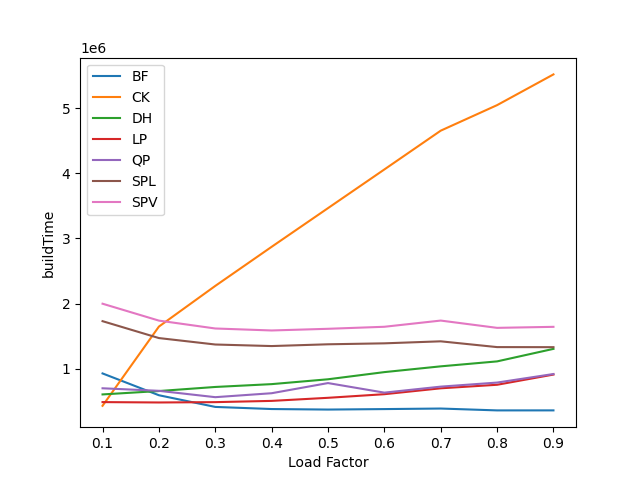
\includegraphics[width=\linewidth]{images/loadFactor_vs_buildTime.png}
          \caption{Build time}\label{fig:plot1}
        \endminipage
        \end{center}
        \end{figure}
    
    As we can see above, the \textit{Cuckoo hashing} is, by far, the slowest algorithm due to its insertion method which can end in cycles; the higher the load factor, the longer the cycles get thus it takes longer to insert a key. \\\\
    Both \textit{Separate chaining} algorithms are the following ones which take longer because when there is an insertion, they may have issues with the memory. The one that performs with a vector may have to relocate all the elements in a given position. The other one just doesn't have the spatial locality principle. \\\\
    On the other hand, the remaining \textit{Open addressing} methods are faster but there is an increment of time as of the load factor. \\\\
    Finally, \textit{Bloom filters} show a little variation but stay almost constant given its implementation. \\\\
    
    From the figures below, we can observe the behaviour performed in ours experiments but we can't extract any significant conclusion regarding the algorithm's implementation. So, we speculate that they are due to the status of the computer.
    
        \begin{figure}[!h]
        \minipage{0.5\textwidth}
          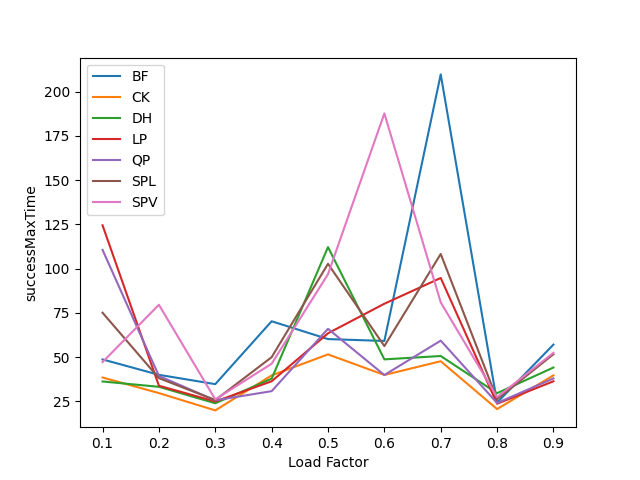
\includegraphics[width=\linewidth]{images/loadFactor_vs_successMaxTime.png}
          \caption{Successful max time}\label{fig:plot2}
        \endminipage\hfill
        \minipage{0.5\textwidth}%
          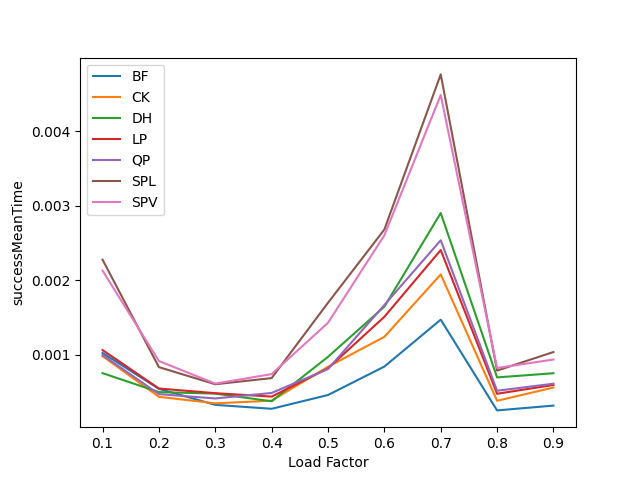
\includegraphics[width=\linewidth]{images/loadFactor_vs_successMeanTime.png}
          \caption{Successful mean time}\label{fig:plot3}
        \endminipage
        \end{figure}
    
    \begin{figure}[!h]
        \minipage{0.5\textwidth}
          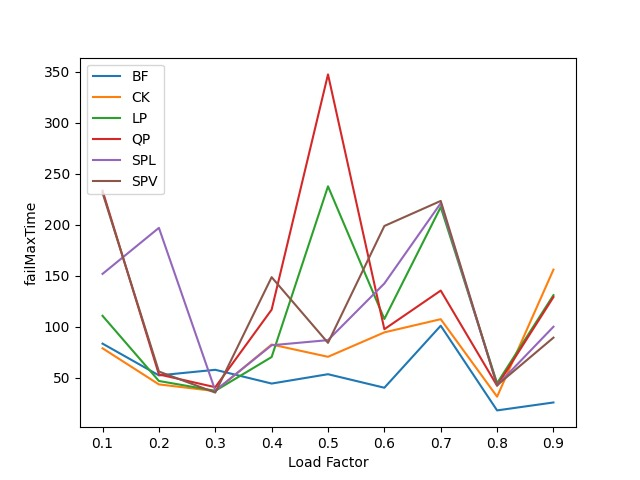
\includegraphics[width=\linewidth]{images/loadFactor_vs_failMaxTime.jpeg}
          \caption{Fail max time}\label{fig:plot2}
        \endminipage\hfill
        \minipage{0.5\textwidth}%
          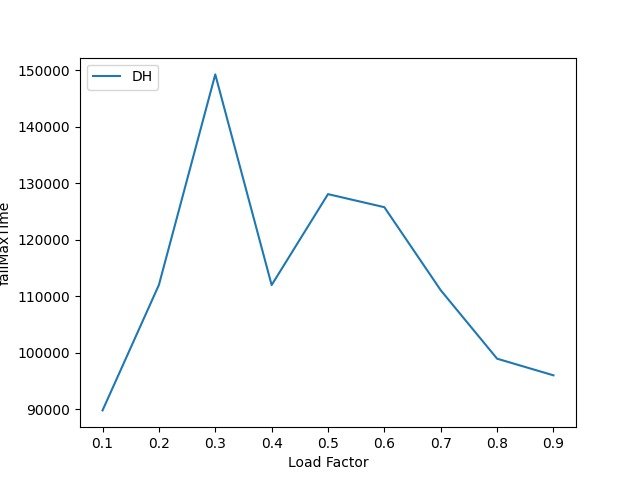
\includegraphics[width=\linewidth]{images/loadFactor_vs_failMaxTimeDH.jpeg}
          \caption{Fail max time}\label{fig:plot3}
        \endminipage
        \end{figure}
        
        \begin{figure}[!h]
        \minipage{0.5\textwidth}
          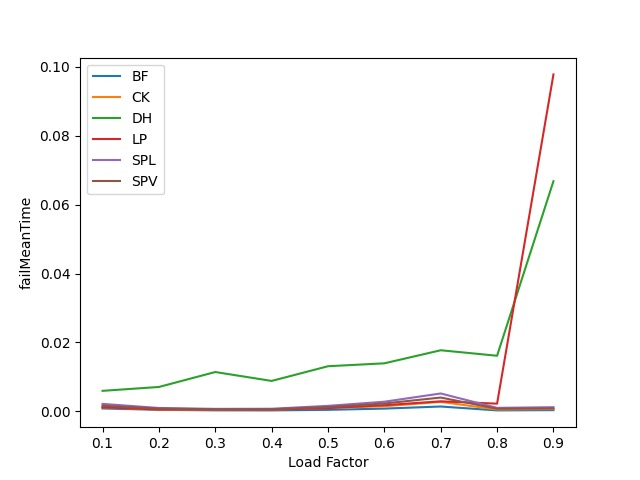
\includegraphics[width=\linewidth]{images/loadFactor_vs_failMeanTime.jpeg}
          \caption{Fail mean time}\label{fig:plot2}
        \endminipage\hfill
        \minipage{0.5\textwidth}%
          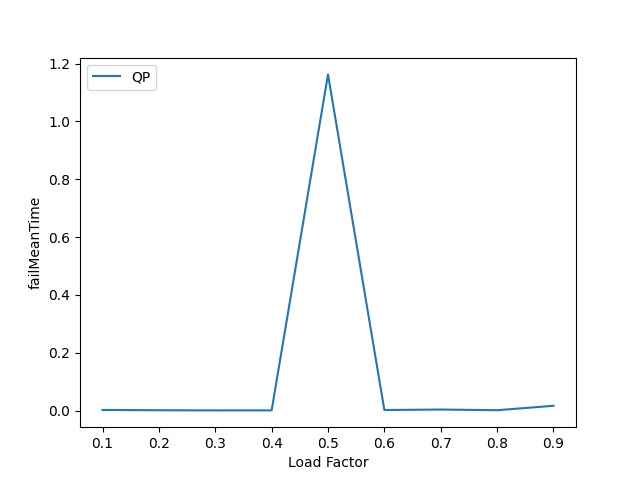
\includegraphics[width=\linewidth]{images/loadFactor_vs_failMeanTimeQP.jpeg}
          \caption{Fail mean time}\label{fig:plot3}
        \endminipage
        \end{figure}
    
    
    \subsection*{Probes metric}
    In this section we compare the average probes that were introduced in each search query regarding the load factor between the experimental values and the theoretical ones.
    
    \subsubsection*{Open Addressing : Linear Probing}
    
        \begin{figure}[!h]
            \minipage{0.5\textwidth}
              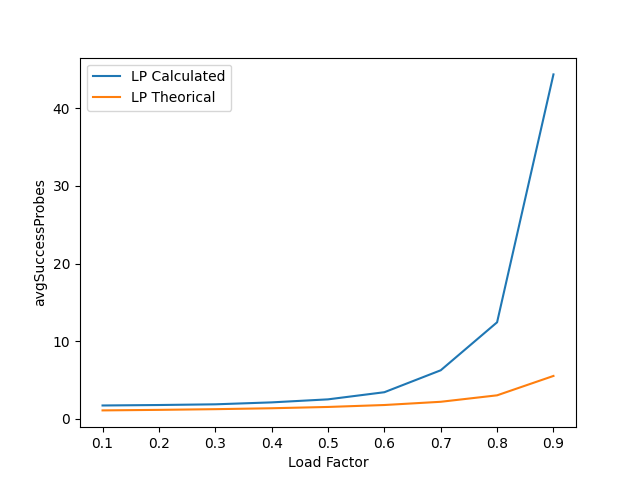
\includegraphics[width=\linewidth]{images/loadFactor_vs_avgSuccessProbes_LP.png}
              \caption{Successful probes}\label{fig:plot4}
            \endminipage\hfill
            \minipage{0.5\textwidth}%
              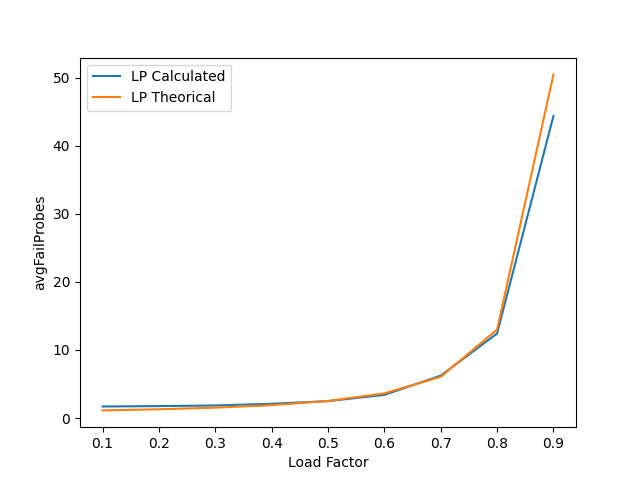
\includegraphics[width=\linewidth]{images/loadFactor_vs_avgFailProbes_LP.png}
              \caption{Fail probes}\label{fig:plot5}
            \endminipage
        \end{figure}
        
    Linear Probing has a similar behaviour in successful queries regarding the theory until $\alpha$ = 0.6, then it start losing the effectively until $\alpha$ = 0.8 when the value soars even though we think 30 probes are not that much.
    Concerning the behaviour in fail queries, it has almost the same performance that the theoretical one.
    
\subsubsection*{Open Addressing : Quadratic Probing}

        \begin{figure}[!h]
    \minipage{0.5\textwidth}
          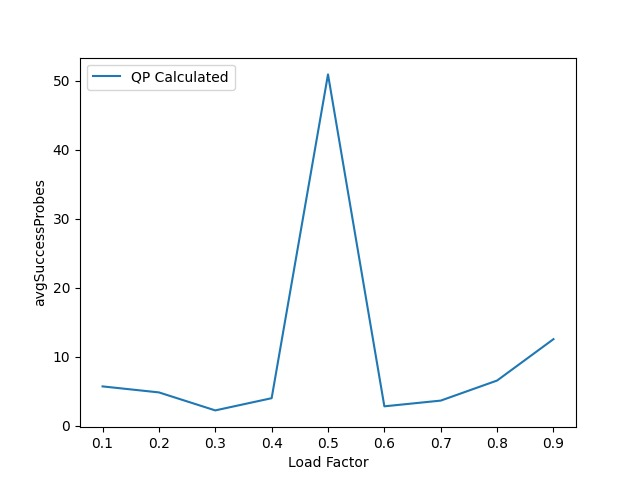
\includegraphics[width=\linewidth]{images/loadFactor_vs_avgSuccessProbes_QP.jpeg}
          \caption{Successful probes}\label{fig:plot6}
        \endminipage\hfill
        \minipage{0.5\textwidth}%
          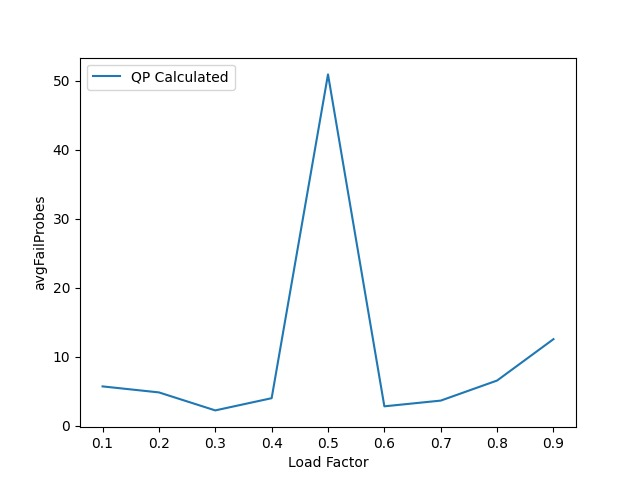
\includegraphics[width=\linewidth]{images/loadFactor_vs_avgFailProbes_QP.jpeg}
          \caption{Fail probes}\label{fig:plot7}
        \endminipage
    \end{figure}
    
    From Quadratic Probing we did not find the theoretical behaviour so we can just comment that the performance done by both successful and fail queries is identical. 
    
    \subsubsection*{Open Addressing : Double Hashing}

        \begin{figure}[!h]
    \minipage{0.5\textwidth}
          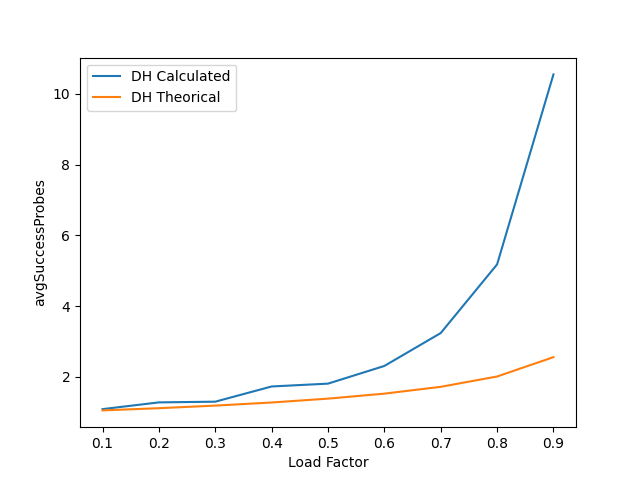
\includegraphics[width=\linewidth]{images/loadFactor_vs_avgSuccessProbes_DH.png}
          \caption{Successful probes}\label{fig:plot8}
        \endminipage\hfill
        \minipage{0.5\textwidth}%
          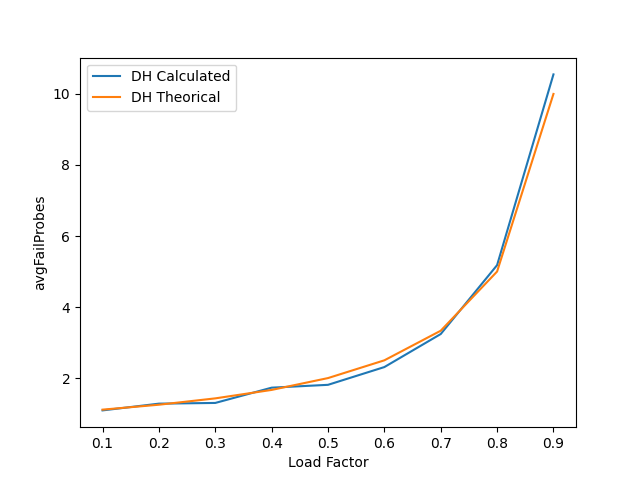
\includegraphics[width=\linewidth]{images/loadFactor_vs_avgFailProbes_DH.png}
          \caption{Fail probes}\label{fig:plot9}
        \endminipage
    \end{figure}
    
    From Double Hashing has a similar behaviour to that of linear probing but better because it need just 10 probes maximum. 
    
    \subsubsection*{Open Addressing : Cuckoo Hashing}

        \begin{figure}[!h]
    \minipage{0.5\textwidth}
          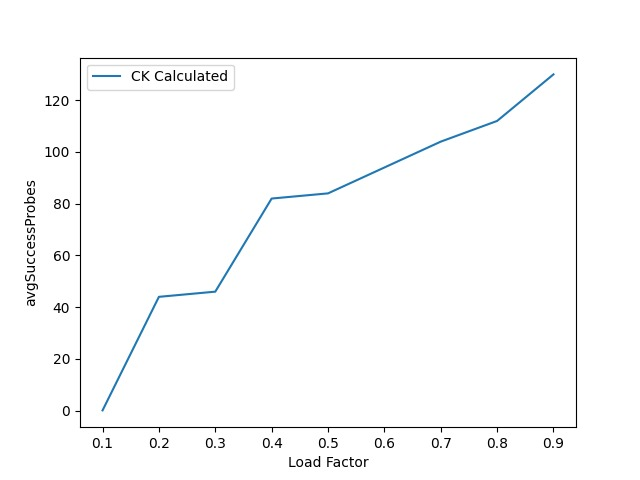
\includegraphics[width=\linewidth]{images/loadFactor_vs_avgSuccessProbes_CK.jpeg}
          \caption{Successful probes}\label{fig:plot10}
        \endminipage\hfill
        \minipage{0.5\textwidth}%
          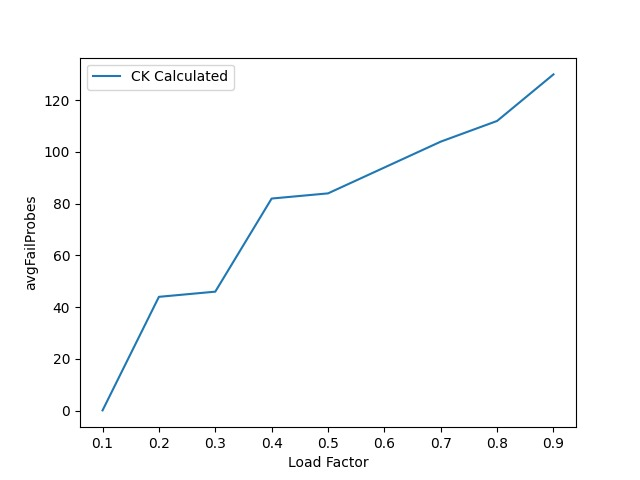
\includegraphics[width=\linewidth]{images/loadFactor_vs_avgFailProbes_CK.jpeg}
          \caption{Fail probes}\label{fig:plot11}
        \endminipage
    \end{figure}
    
    From Cuckoo Hashing we did not find the theoretical behaviour so we can just comment that the performance done by both successful and fail queries is identical. The bad conduct is due to the inner cycles that have its implementation.
    
    \subsubsection*{Separate Chaining}

        \begin{figure}[!h]
    \minipage{0.5\textwidth}
          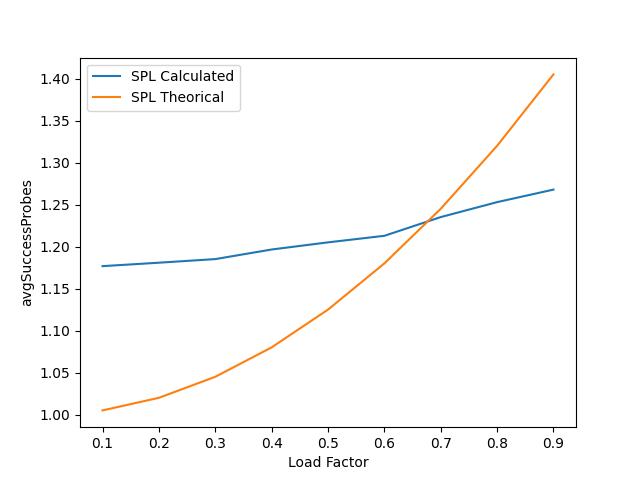
\includegraphics[width=\linewidth]{images/loadFactor_vs_avgSuccessProbes_SPL.png}
          \caption{Successful probes}\label{fig:plot12}
        \endminipage\hfill
        \minipage{0.5\textwidth}%
          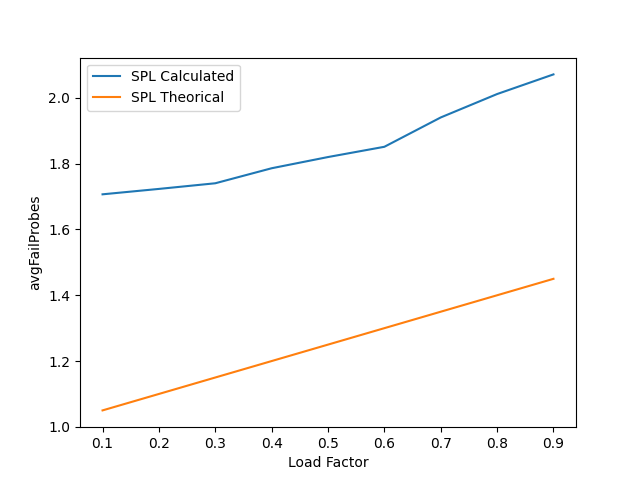
\includegraphics[width=\linewidth]{images/loadFactor_vs_avgFailProbes_SPL.png}
          \caption{Fail probes}\label{fig:plot13}
        \endminipage
    \end{figure}

        \begin{figure}[!h]
    \minipage{0.5\textwidth}
          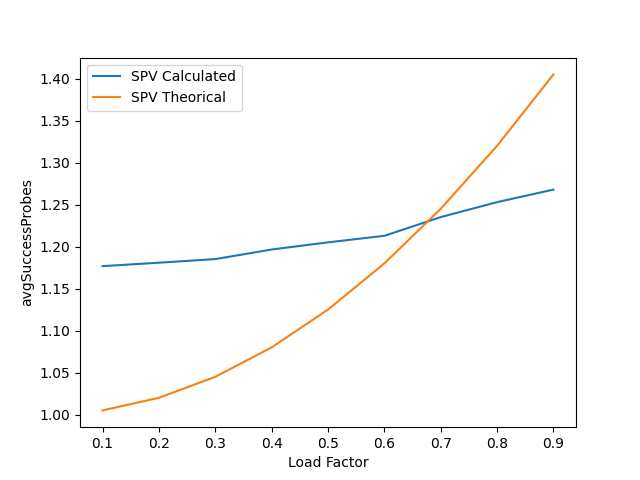
\includegraphics[width=\linewidth]{images/loadFactor_vs_avgSuccessProbes_SPV.png}
          \caption{Successful probes}\label{fig:plot14}
        \endminipage\hfill
        \minipage{0.5\textwidth}%
          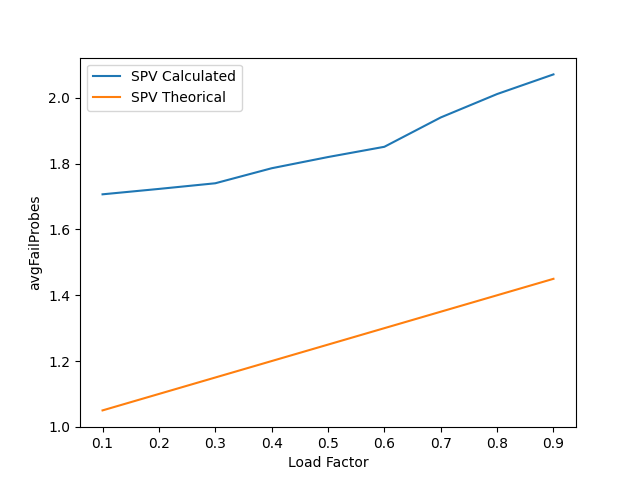
\includegraphics[width=\linewidth]{images/loadFactor_vs_avgFailProbes_SPV.png}
          \caption{Fail probes}\label{fig:plot15}
        \endminipage
    \end{figure}
    
    From all Separate Chaining's plots, we can observe that with both queries, with lower load factor we get less collisions and this decreases the number of accesses needed. As the load factor increases, the number of collisions also increases and as we have no repetitions, it becomes harder to find the value in the first search in the vector or list. Also, we can observe that all plots have a growing trend but with a vertical displacement that we attribute to the conditions of the experiment and the implementations of the algorithms.
    
    \subsection*{False positives}
        This section is specifically centred in the false positive rate of the bloom filters since the other techniques do not have. \\\\
        Both plots have a similar figure but in this case the experimental results show a much better performance with a lower false positive rate. 
        
        \begin{figure}[!h]
        \begin{center}
        \minipage{0.5\textwidth}
          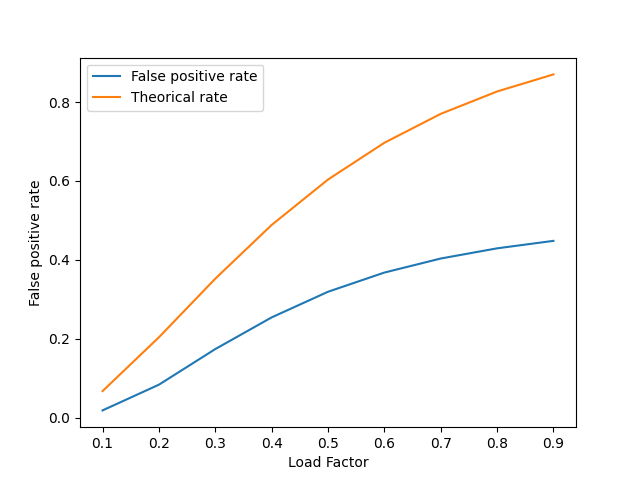
\includegraphics[width=\linewidth]{images/loadFactor_vs_falsePositives.png}
          \caption{False positive rate comparison}\label{fig:plot16}
        \endminipage
        \end{center}
        \end{figure}

\section{Discussion}
Along this research work we found out that no matter the implementation all techniques have a similar lookup time. \\
On the other hand the implementation does affect the build time and, as we have seen with the experiment results, \textit{bloom filters} is the one that performs faster; unfortunately it has the issue of \textit{false positives}. \\\\
Furthermore, in this project we have learnt how to design experiments, collect data, extract results and conclusions. We also have learnt teamwork and the fair use of collaborative tools such as git and overleaf. \\\\
Finally we wanted to add that we have struggled so many hours with LaTeX, the position of the plots and its compilation errors.


    \printbibliography

\end{document}
